% Options for packages loaded elsewhere
% Options for packages loaded elsewhere
\PassOptionsToPackage{unicode}{hyperref}
\PassOptionsToPackage{hyphens}{url}
\PassOptionsToPackage{dvipsnames,svgnames,x11names}{xcolor}
%
\documentclass[
  portuguese,
  letterpaper,
  DIV=11,
  numbers=noendperiod]{scrartcl}
\usepackage{xcolor}
\usepackage{amsmath,amssymb}
\setcounter{secnumdepth}{-\maxdimen} % remove section numbering
\usepackage{iftex}
\ifPDFTeX
  \usepackage[T1]{fontenc}
  \usepackage[utf8]{inputenc}
  \usepackage{textcomp} % provide euro and other symbols
\else % if luatex or xetex
  \usepackage{unicode-math} % this also loads fontspec
  \defaultfontfeatures{Scale=MatchLowercase}
  \defaultfontfeatures[\rmfamily]{Ligatures=TeX,Scale=1}
\fi
\usepackage{lmodern}
\ifPDFTeX\else
  % xetex/luatex font selection
\fi
% Use upquote if available, for straight quotes in verbatim environments
\IfFileExists{upquote.sty}{\usepackage{upquote}}{}
\IfFileExists{microtype.sty}{% use microtype if available
  \usepackage[]{microtype}
  \UseMicrotypeSet[protrusion]{basicmath} % disable protrusion for tt fonts
}{}
\makeatletter
\@ifundefined{KOMAClassName}{% if non-KOMA class
  \IfFileExists{parskip.sty}{%
    \usepackage{parskip}
  }{% else
    \setlength{\parindent}{0pt}
    \setlength{\parskip}{6pt plus 2pt minus 1pt}}
}{% if KOMA class
  \KOMAoptions{parskip=half}}
\makeatother
% Make \paragraph and \subparagraph free-standing
\makeatletter
\ifx\paragraph\undefined\else
  \let\oldparagraph\paragraph
  \renewcommand{\paragraph}{
    \@ifstar
      \xxxParagraphStar
      \xxxParagraphNoStar
  }
  \newcommand{\xxxParagraphStar}[1]{\oldparagraph*{#1}\mbox{}}
  \newcommand{\xxxParagraphNoStar}[1]{\oldparagraph{#1}\mbox{}}
\fi
\ifx\subparagraph\undefined\else
  \let\oldsubparagraph\subparagraph
  \renewcommand{\subparagraph}{
    \@ifstar
      \xxxSubParagraphStar
      \xxxSubParagraphNoStar
  }
  \newcommand{\xxxSubParagraphStar}[1]{\oldsubparagraph*{#1}\mbox{}}
  \newcommand{\xxxSubParagraphNoStar}[1]{\oldsubparagraph{#1}\mbox{}}
\fi
\makeatother

\usepackage{color}
\usepackage{fancyvrb}
\newcommand{\VerbBar}{|}
\newcommand{\VERB}{\Verb[commandchars=\\\{\}]}
\DefineVerbatimEnvironment{Highlighting}{Verbatim}{commandchars=\\\{\}}
% Add ',fontsize=\small' for more characters per line
\usepackage{framed}
\definecolor{shadecolor}{RGB}{241,243,245}
\newenvironment{Shaded}{\begin{snugshade}}{\end{snugshade}}
\newcommand{\AlertTok}[1]{\textcolor[rgb]{0.68,0.00,0.00}{#1}}
\newcommand{\AnnotationTok}[1]{\textcolor[rgb]{0.37,0.37,0.37}{#1}}
\newcommand{\AttributeTok}[1]{\textcolor[rgb]{0.40,0.45,0.13}{#1}}
\newcommand{\BaseNTok}[1]{\textcolor[rgb]{0.68,0.00,0.00}{#1}}
\newcommand{\BuiltInTok}[1]{\textcolor[rgb]{0.00,0.23,0.31}{#1}}
\newcommand{\CharTok}[1]{\textcolor[rgb]{0.13,0.47,0.30}{#1}}
\newcommand{\CommentTok}[1]{\textcolor[rgb]{0.37,0.37,0.37}{#1}}
\newcommand{\CommentVarTok}[1]{\textcolor[rgb]{0.37,0.37,0.37}{\textit{#1}}}
\newcommand{\ConstantTok}[1]{\textcolor[rgb]{0.56,0.35,0.01}{#1}}
\newcommand{\ControlFlowTok}[1]{\textcolor[rgb]{0.00,0.23,0.31}{\textbf{#1}}}
\newcommand{\DataTypeTok}[1]{\textcolor[rgb]{0.68,0.00,0.00}{#1}}
\newcommand{\DecValTok}[1]{\textcolor[rgb]{0.68,0.00,0.00}{#1}}
\newcommand{\DocumentationTok}[1]{\textcolor[rgb]{0.37,0.37,0.37}{\textit{#1}}}
\newcommand{\ErrorTok}[1]{\textcolor[rgb]{0.68,0.00,0.00}{#1}}
\newcommand{\ExtensionTok}[1]{\textcolor[rgb]{0.00,0.23,0.31}{#1}}
\newcommand{\FloatTok}[1]{\textcolor[rgb]{0.68,0.00,0.00}{#1}}
\newcommand{\FunctionTok}[1]{\textcolor[rgb]{0.28,0.35,0.67}{#1}}
\newcommand{\ImportTok}[1]{\textcolor[rgb]{0.00,0.46,0.62}{#1}}
\newcommand{\InformationTok}[1]{\textcolor[rgb]{0.37,0.37,0.37}{#1}}
\newcommand{\KeywordTok}[1]{\textcolor[rgb]{0.00,0.23,0.31}{\textbf{#1}}}
\newcommand{\NormalTok}[1]{\textcolor[rgb]{0.00,0.23,0.31}{#1}}
\newcommand{\OperatorTok}[1]{\textcolor[rgb]{0.37,0.37,0.37}{#1}}
\newcommand{\OtherTok}[1]{\textcolor[rgb]{0.00,0.23,0.31}{#1}}
\newcommand{\PreprocessorTok}[1]{\textcolor[rgb]{0.68,0.00,0.00}{#1}}
\newcommand{\RegionMarkerTok}[1]{\textcolor[rgb]{0.00,0.23,0.31}{#1}}
\newcommand{\SpecialCharTok}[1]{\textcolor[rgb]{0.37,0.37,0.37}{#1}}
\newcommand{\SpecialStringTok}[1]{\textcolor[rgb]{0.13,0.47,0.30}{#1}}
\newcommand{\StringTok}[1]{\textcolor[rgb]{0.13,0.47,0.30}{#1}}
\newcommand{\VariableTok}[1]{\textcolor[rgb]{0.07,0.07,0.07}{#1}}
\newcommand{\VerbatimStringTok}[1]{\textcolor[rgb]{0.13,0.47,0.30}{#1}}
\newcommand{\WarningTok}[1]{\textcolor[rgb]{0.37,0.37,0.37}{\textit{#1}}}

\usepackage{longtable,booktabs,array}
\usepackage{calc} % for calculating minipage widths
% Correct order of tables after \paragraph or \subparagraph
\usepackage{etoolbox}
\makeatletter
\patchcmd\longtable{\par}{\if@noskipsec\mbox{}\fi\par}{}{}
\makeatother
% Allow footnotes in longtable head/foot
\IfFileExists{footnotehyper.sty}{\usepackage{footnotehyper}}{\usepackage{footnote}}
\makesavenoteenv{longtable}
\usepackage{graphicx}
\makeatletter
\newsavebox\pandoc@box
\newcommand*\pandocbounded[1]{% scales image to fit in text height/width
  \sbox\pandoc@box{#1}%
  \Gscale@div\@tempa{\textheight}{\dimexpr\ht\pandoc@box+\dp\pandoc@box\relax}%
  \Gscale@div\@tempb{\linewidth}{\wd\pandoc@box}%
  \ifdim\@tempb\p@<\@tempa\p@\let\@tempa\@tempb\fi% select the smaller of both
  \ifdim\@tempa\p@<\p@\scalebox{\@tempa}{\usebox\pandoc@box}%
  \else\usebox{\pandoc@box}%
  \fi%
}
% Set default figure placement to htbp
\def\fps@figure{htbp}
\makeatother


% definitions for citeproc citations
\NewDocumentCommand\citeproctext{}{}
\NewDocumentCommand\citeproc{mm}{%
  \begingroup\def\citeproctext{#2}\cite{#1}\endgroup}
\makeatletter
 % allow citations to break across lines
 \let\@cite@ofmt\@firstofone
 % avoid brackets around text for \cite:
 \def\@biblabel#1{}
 \def\@cite#1#2{{#1\if@tempswa , #2\fi}}
\makeatother
\newlength{\cslhangindent}
\setlength{\cslhangindent}{1.5em}
\newlength{\csllabelwidth}
\setlength{\csllabelwidth}{3em}
\newenvironment{CSLReferences}[2] % #1 hanging-indent, #2 entry-spacing
 {\begin{list}{}{%
  \setlength{\itemindent}{0pt}
  \setlength{\leftmargin}{0pt}
  \setlength{\parsep}{0pt}
  % turn on hanging indent if param 1 is 1
  \ifodd #1
   \setlength{\leftmargin}{\cslhangindent}
   \setlength{\itemindent}{-1\cslhangindent}
  \fi
  % set entry spacing
  \setlength{\itemsep}{#2\baselineskip}}}
 {\end{list}}
\usepackage{calc}
\newcommand{\CSLBlock}[1]{\hfill\break\parbox[t]{\linewidth}{\strut\ignorespaces#1\strut}}
\newcommand{\CSLLeftMargin}[1]{\parbox[t]{\csllabelwidth}{\strut#1\strut}}
\newcommand{\CSLRightInline}[1]{\parbox[t]{\linewidth - \csllabelwidth}{\strut#1\strut}}
\newcommand{\CSLIndent}[1]{\hspace{\cslhangindent}#1}

\ifLuaTeX
\usepackage[bidi=basic]{babel}
\else
\usepackage[bidi=default]{babel}
\fi
% get rid of language-specific shorthands (see #6817):
\let\LanguageShortHands\languageshorthands
\def\languageshorthands#1{}


\setlength{\emergencystretch}{3em} % prevent overfull lines

\providecommand{\tightlist}{%
  \setlength{\itemsep}{0pt}\setlength{\parskip}{0pt}}



 


\KOMAoption{captions}{tableheading}
\makeatletter
\@ifpackageloaded{caption}{}{\usepackage{caption}}
\AtBeginDocument{%
\ifdefined\contentsname
  \renewcommand*\contentsname{Índice}
\else
  \newcommand\contentsname{Índice}
\fi
\ifdefined\listfigurename
  \renewcommand*\listfigurename{Lista de Figuras}
\else
  \newcommand\listfigurename{Lista de Figuras}
\fi
\ifdefined\listtablename
  \renewcommand*\listtablename{Lista de Tabelas}
\else
  \newcommand\listtablename{Lista de Tabelas}
\fi
\ifdefined\figurename
  \renewcommand*\figurename{Figura}
\else
  \newcommand\figurename{Figura}
\fi
\ifdefined\tablename
  \renewcommand*\tablename{Tabela}
\else
  \newcommand\tablename{Tabela}
\fi
}
\@ifpackageloaded{float}{}{\usepackage{float}}
\floatstyle{ruled}
\@ifundefined{c@chapter}{\newfloat{codelisting}{h}{lop}}{\newfloat{codelisting}{h}{lop}[chapter]}
\floatname{codelisting}{Listagem}
\newcommand*\listoflistings{\listof{codelisting}{Lista de Listagens}}
\makeatother
\makeatletter
\makeatother
\makeatletter
\@ifpackageloaded{caption}{}{\usepackage{caption}}
\@ifpackageloaded{subcaption}{}{\usepackage{subcaption}}
\makeatother
\usepackage{bookmark}
\IfFileExists{xurl.sty}{\usepackage{xurl}}{} % add URL line breaks if available
\urlstyle{same}
\hypersetup{
  pdftitle={Um Exemplo Prático com Quarto: A Distribuição de Poisson},
  pdfauthor={Prof.~Dr.~Sadraque E. F. Lucena},
  pdflang={pt},
  colorlinks=true,
  linkcolor={blue},
  filecolor={Maroon},
  citecolor={Blue},
  urlcolor={Blue},
  pdfcreator={LaTeX via pandoc}}


\title{Um Exemplo Prático com Quarto: A Distribuição de Poisson}
\author{Prof.~Dr.~Sadraque E. F. Lucena}
\date{}
\begin{document}
\maketitle


Este é um arquivo usado como exemplo na disciplina ESTAT0109 - Mineração
de Dados em Estatística, com o intuito de explorar a aplicação do
Quarto, uma ferramenta de publicação técnica de código aberto projetada
para auxiliar os cientistas de dados na compartilhamento de suas
análises. Como exemplo, realizaremos uma breve exploração da
distribuição de Poisson.

\subsection{A distribuição de
Poisson}\label{a-distribuiuxe7uxe3o-de-poisson}

A distribuição de Poisson é uma distribuição de probabilidade discreta
que descreve o número de eventos que ocorrem em um intervalo fixo de
tempo ou espaço. A distribuição de Poisson é frequentemente utilizada em
problemas do mundo real, como prever o número de chamadas recebidas em
um \emph{call center} em uma hora, o número de defeitos em um lote de
produtos, ou a contagem de eventos raros em geral.

\subsection{A Fórmula Matemática}\label{a-fuxf3rmula-matemuxe1tica}

Seja \(X\) uma variável aleatória com distribuição de Poisson com
parâmetro \(\lambda\), denotada como \(X\sim Poisson(\lambda)\). A
função de probabilidade de \(X\) é então dada por (MORETTIN; BUSSAB,
2017)

\[
  P(X=x) = \frac{e^{-\lambda}\lambda^x}{x!},
\] onde:

\begin{itemize}
\tightlist
\item
  \(e\) é a função exponencial;
\item
  \(x\) é o número de ocorrências de um evento (\(x=0, 1, 2, \ldots\)).
\item
  \(\lambda\) (lambda) é um número real positivo que representa a média
  de ocorrências no intervalo especificado.
\end{itemize}

\subsection{Exemplo Prático de
Aplicação}\label{exemplo-pruxe1tico-de-aplicauxe7uxe3o}

Vamos imaginar algumas situações onde a Poisson se aplica. A
Tabela~\ref{tbl-letters}, criada com a sintaxe simples do Markdown, nos
dá alguns exemplos:

\begin{longtable}[]{@{}
  >{\raggedright\arraybackslash}p{(\linewidth - 4\tabcolsep) * \real{0.5321}}
  >{\centering\arraybackslash}p{(\linewidth - 4\tabcolsep) * \real{0.1927}}
  >{\raggedleft\arraybackslash}p{(\linewidth - 4\tabcolsep) * \real{0.2752}}@{}}
\caption{Exemplos de aplicação da distribuição de
Poisson.}\label{tbl-letters}\tabularnewline
\toprule\noalign{}
\begin{minipage}[b]{\linewidth}\raggedright
Fenômeno Observado
\end{minipage} & \begin{minipage}[b]{\linewidth}\centering
Intervalo
\end{minipage} & \begin{minipage}[b]{\linewidth}\raggedleft
Valor de Lambda (\(\lambda\))
\end{minipage} \\
\midrule\noalign{}
\endfirsthead
\toprule\noalign{}
\begin{minipage}[b]{\linewidth}\raggedright
Fenômeno Observado
\end{minipage} & \begin{minipage}[b]{\linewidth}\centering
Intervalo
\end{minipage} & \begin{minipage}[b]{\linewidth}\raggedleft
Valor de Lambda (\(\lambda\))
\end{minipage} \\
\midrule\noalign{}
\endhead
\bottomrule\noalign{}
\endlastfoot
Carros passando por um cruzamento & 1 minuto & 10 \\
Erros de digitação em uma página de um livro & Por página & 2 \\
Gols marcados em uma partida de futebol & Por partida & 2.5 \\
\end{longtable}

\subsection{Simulando e Visualizando Dados da Poisson em
R}\label{simulando-e-visualizando-dados-da-poisson-em-r}

Agora, a mágica do Quarto: vamos usar um bloco (\emph{chunk}) de código
R para simular dados de uma distribuição de Poisson e visualizá-los.
Vamos simular 1000 observações de uma Poisson com \(\lambda = 5\).
Usaremos o pacote \texttt{ggplot2} para criar um histograma elegante.

\begin{Shaded}
\begin{Highlighting}[]
\CommentTok{\# 1. Carregar o pacote ggplot2 para visualização}
\FunctionTok{library}\NormalTok{(ggplot2)}

\CommentTok{\# 2. Definir o nosso parâmetro lambda}
\NormalTok{lambda\_valor }\OtherTok{\textless{}{-}} \DecValTok{5}

\CommentTok{\# 3. Gerar 1000 números aleatórios de uma distribuição Poisson}
\NormalTok{dados\_poisson }\OtherTok{\textless{}{-}} \FunctionTok{rpois}\NormalTok{(}\AttributeTok{n =} \DecValTok{1000}\NormalTok{, }\AttributeTok{lambda =}\NormalTok{ lambda\_valor)}

\CommentTok{\# 4. Criar o histograma}
\FunctionTok{ggplot}\NormalTok{(}\AttributeTok{data =} \FunctionTok{data.frame}\NormalTok{(}\AttributeTok{dados =}\NormalTok{ dados\_poisson), }\FunctionTok{aes}\NormalTok{(}\AttributeTok{x =}\NormalTok{ dados)) }\SpecialCharTok{+}
  \FunctionTok{geom\_histogram}\NormalTok{(}\AttributeTok{binwidth =} \DecValTok{1}\NormalTok{, }\AttributeTok{fill =} \StringTok{"skyblue"}\NormalTok{, }\AttributeTok{color =} \StringTok{"black"}\NormalTok{, }\AttributeTok{alpha =} \FloatTok{0.8}\NormalTok{) }\SpecialCharTok{+}
  \FunctionTok{labs}\NormalTok{(}
    \AttributeTok{title =} \StringTok{"Distribuição de 1000 Observações de uma Poisson"}\NormalTok{,}
    \AttributeTok{subtitle =} \FunctionTok{paste}\NormalTok{(}\StringTok{"Lambda (taxa média) ="}\NormalTok{, lambda\_valor),}
    \AttributeTok{x =} \StringTok{"Número de Eventos (x)"}\NormalTok{,}
    \AttributeTok{y =} \StringTok{"Frequência"}
\NormalTok{  ) }\SpecialCharTok{+}
  \FunctionTok{theme\_minimal}\NormalTok{()}
\end{Highlighting}
\end{Shaded}

\begin{figure}[H]

\centering{

\pandocbounded{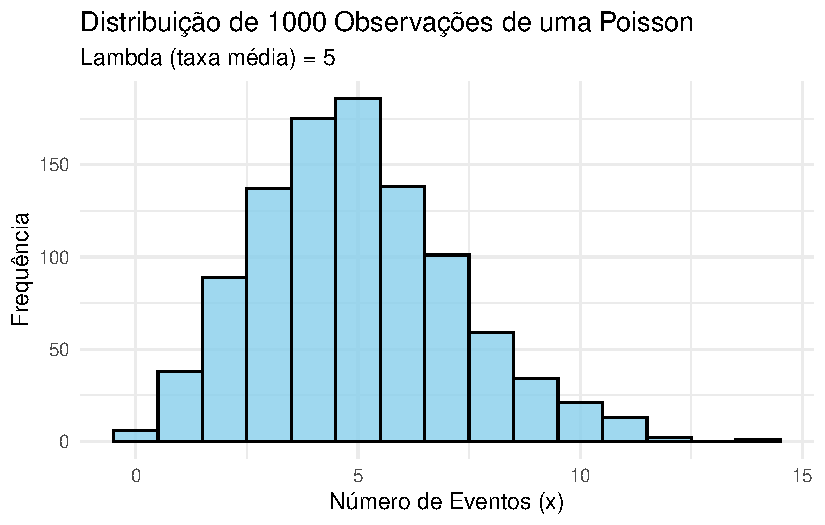
\includegraphics[keepaspectratio]{arquivo-exemplo-quarto_files/figure-pdf/fig-gerar-e-plotar-poisson-1.pdf}}

}

\caption{\label{fig-gerar-e-plotar-poisson}Histograma de 1000 valores
simulados de uma distribuição de Poisson com lambda = 5.}

\end{figure}%

Como podemos ver na Figura~\ref{fig-gerar-e-plotar-poisson}, a maior
parte dos nossos dados se concentra em torno do valor de lambda, que é
5.

\subsection{Tabela de Estatísticas
Descritivas}\label{tabela-de-estatuxedsticas-descritivas}

Para complementar nossa análise, podemos criar uma tabela de resumo
profissional dos dados simulados. Usaremos o pacote \texttt{gtsummary},
que é fantástico para criar tabelas prontas para publicação com um
código muito simples.

\begin{Shaded}
\begin{Highlighting}[]
\FunctionTok{library}\NormalTok{(knitr)}
\NormalTok{resumo\_df }\OtherTok{\textless{}{-}} \FunctionTok{data.frame}\NormalTok{(}
  \StringTok{"Estatística"} \OtherTok{=} \FunctionTok{c}\NormalTok{(}\StringTok{"Tamanho da Amostra (n)"}\NormalTok{,}
                  \StringTok{"Valor Mínimo"}\NormalTok{,}
                  \StringTok{"Valor Máximo"}\NormalTok{,}
                  \StringTok{"Média"}\NormalTok{,}
                  \StringTok{"Variância"}\NormalTok{),}
  \AttributeTok{Valor =} \FunctionTok{c}\NormalTok{(}
    \FunctionTok{length}\NormalTok{(dados\_poisson),}
    \FunctionTok{min}\NormalTok{(dados\_poisson),}
    \FunctionTok{max}\NormalTok{(dados\_poisson),}
    \FunctionTok{mean}\NormalTok{(dados\_poisson),}
    \FunctionTok{var}\NormalTok{(dados\_poisson)}
\NormalTok{  )}
\NormalTok{)}
\FunctionTok{kable}\NormalTok{(resumo\_df,}
      \AttributeTok{caption =} \StringTok{"Estatísticas Descritivas dos Dados Simulados"}\NormalTok{,}
      \AttributeTok{digits =} \DecValTok{2}\NormalTok{)}
\end{Highlighting}
\end{Shaded}

\begin{longtable}[]{@{}lr@{}}

\caption{\label{tbl-resumo}Estatísticas Descritivas dos Dados Simulados}

\tabularnewline

\toprule\noalign{}
Estatística & Valor \\
\midrule\noalign{}
\endhead
\bottomrule\noalign{}
\endlastfoot
Tamanho da Amostra (n) & 1000.00 \\
Valor Mínimo & 0.00 \\
Valor Máximo & 14.00 \\
Média & 4.96 \\
Variância & 5.07 \\

\end{longtable}

A Tabela~\ref{tbl-resumo} acima confirma o que esperávamos: a média e a
variância dos nossos dados simulados são muito próximas de
\(\lambda=5\).

\section*{Referências}\label{referuxeancias}
\addcontentsline{toc}{section}{Referências}

\phantomsection\label{refs}
\begin{CSLReferences}{0}{1}
\bibitem[\citeproctext]{ref-morettin2017estatistica}
MORETTIN, P. A.; BUSSAB, W. O. \textbf{Estat{ı́}stica b{á}sica}. 9. ed.
São Paulo: Saraiva, 2017.

\end{CSLReferences}




\end{document}
